\documentclass[10pt,aspectratio=169]{beamer}
\usetheme[progressbar=frametitle]{metropolis}
\usepackage{appendixnumberbeamer}
\usepackage{cancel}
\setbeamercolor{background canvas}{bg=white}
\usepackage{booktabs}
\usepackage{drawmatrix}
\usetikzlibrary{positioning}

\usepackage{fontawesome} % requires XeTeX or LuaTeX


% \usepackage[scale=2]{ccicons}
% \usepackage{eulervm}
\usepackage{pgfplots}
\usepackage{xspace}
\DeclareSymbolFont{sfoperators}{OT1}{FiraSans-LF}{l}{n}
\makeatletter
    \renewcommand{\operator@font}{\mathgroup\symsfoperators}
\makeatother
\DeclareMathOperator*{\argmin}{arg\,min}
\metroset{block=fill}

\title{Variational DA and ML}
\subtitle{Using ML-based preconditioners in VarDA problems}
\date{\today}% \\ \emph{AIRSEA Working Group}}
\author{Victor Trappler}
\institute{
    \begin{center}
        
\includegraphics[height=.8cm]{img/Atos_logo.png}
        \hspace{0.3cm}
        
\includegraphics[height=.8cm]{img/Inria_logo.png}
    \end{center}
}



\begin{document}

\begin{frame}{Current work}

\begin{block}{The Problem we are trying to solve}
Solve for $\tilde{x}$:
\begin{equation}     
    A(x)\tilde{x} = b(x)
    \end{equation}
    with $A(x) = \left(B^{-1} + (HM)^TR^{-1} (HM)\right)$
\end{block}
\begin{itemize}
    \item Learn a low-rank approximation using DNN (to use as preconditioner):
    \begin{itemize}
        \item $x \mapsto (U(x), S(x)) \in \mathbb{R}^{n \times r} \times \mathbb{R}^r$ where 
        $A(x) \approx U(x)\mathrm{diag}(S(x)) U(x)^T$
        \item Approximate the norm using random vectors
        \item Look for an approximation in the dual space instead ?
    \end{itemize}
    \item Better architecture for neural network (CNN, UNet, attention layers?), instead of MLP
    \item (Technical stuff): DVC and MLflow for reproductibility, data versioning and workflow management
\end{itemize}
\end{frame}

\maketitle
\begin{frame}{Table of contents}
  \setbeamertemplate{section in toc}[sections numbered]
  \tableofcontents%[hideallsubsections]
\end{frame}

\section{Introduction}
\begin{frame}{Notation and setting}
\begin{itemize}
    \item $x \in \mathbb{R}^n$ state vector: Variables that describe a physical system ($n = \mathcal{O}(10^{6-9})$) 
\end{itemize}
    Different sources of information on a state vector $x$:
    \begin{itemize}
        \item A priori information $p(x)$
        \begin{itemize}
            \item Historical data
            \item Balance equations
        \end{itemize}
        \item Observations $y$, obtained more or less indirectly
        \item Numerical model which maps the state to the observations $\mathcal{G} = \mathcal{H} \circ \mathcal{M}$
    \end{itemize}
    How to combine them ? Bayes theorem
\end{frame}


\begin{frame}{Data Assimilation and Bayesian Inference}
Bayes' theorem \only<2>{sequentially}: update information on \only<1>{$x$ using $y$ } \only<2>{$x_t$ using $y_t$}
\only<1>{
\begin{equation}
 \alert{p(x \mid y)} = \alert{p(x)} \frac{\overbrace{p(y \mid x)}^{\text{likelihood}}}{\underbrace{p(y)}_{\text{evidence}}}
\end{equation}}
\only<2>{
\begin{equation}
     \alert{p(x_t \mid y_{t})} = \underbrace{\alert{p(x_t \mid x_{t-1})}}_{prior/forecast} \frac{\overbrace{p(y_t \mid x_t)}^{\text{likelihood}}}{\underbrace{p(y_t)}_{\text{evidence}}}
\end{equation}
}
\begin{center}
    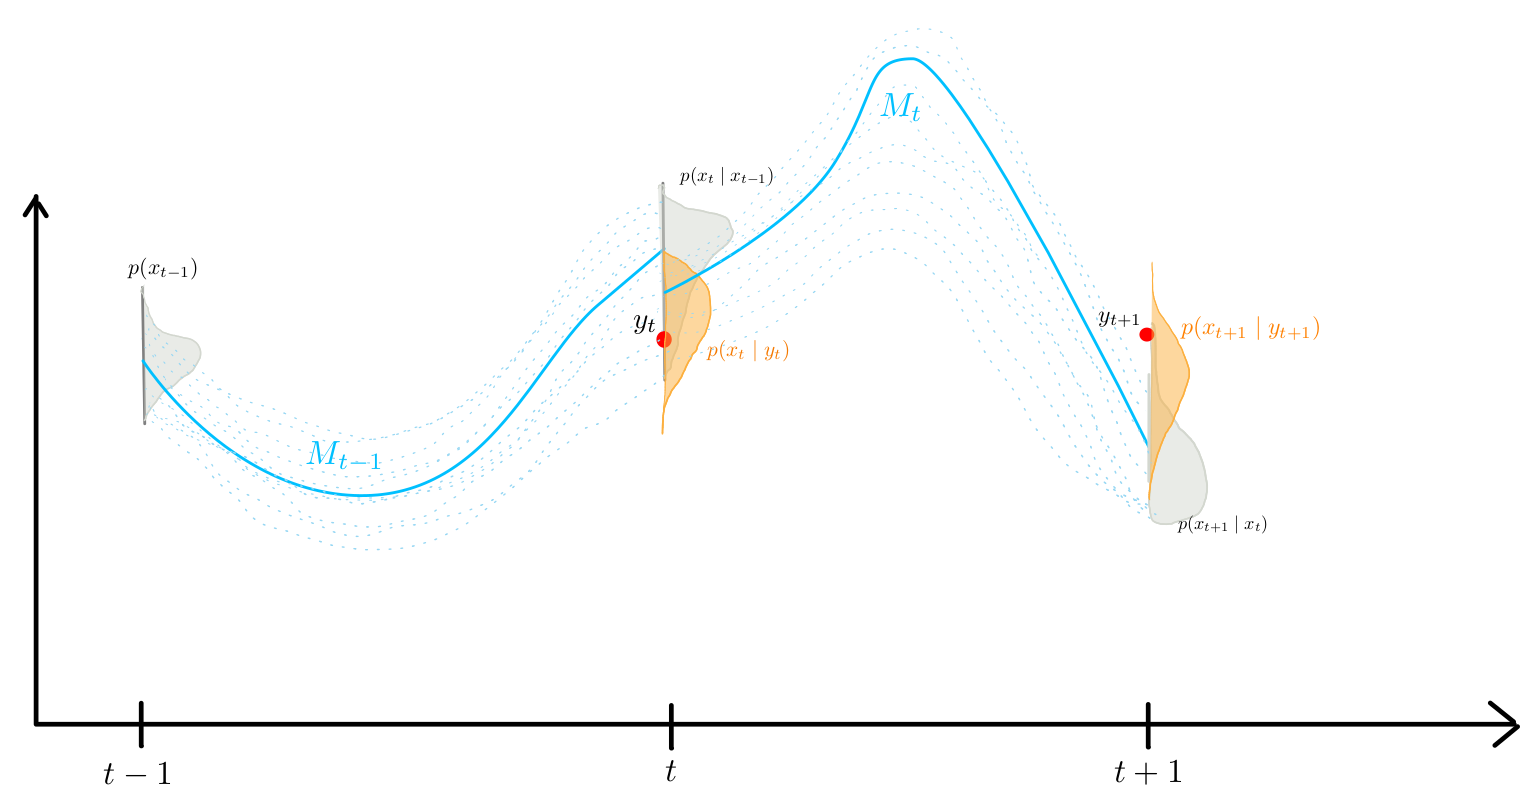
\includegraphics[height=.6\textheight]{img/Bayes_DA.png}
\end{center}
\end{frame}

\section{Variational Data Assimilation}
\begin{frame}{Point estimates}
    We are interested in a point estimate of the posterior distribution: \alert{M}aximum \alert{A P}osteriori 
    \begin{equation}
        \min_x \{ -\log p(x \mid y) \} =\min_x\{ - \underbrace{\log p(y\mid x)}_{\text{log-lik=misfit}} - \underbrace{\log p(x)}_{\text{regularization}} \}
    \end{equation}
         \begin{itemize}
          \item $Y \mid x$ encodes the relation between the forward model and the observations
          \item $X$ encodes the knowledge we gathered so far on $x$ 
      \end{itemize}
    \begin{block}{Gaussian Assumptions}
 \begin{itemize}
     \item $y = \mathcal{G}(x) + \varepsilon$, then $Y \mid x \sim\mathcal{N}(\mathcal{G}(x), R)$ 
     \item $x \sim \mathcal{N}(x^b, B)$
 \end{itemize}
    \end{block}
\end{frame}



\begin{frame}{Standard formulation of the objective function}
Using the Gaussian assumptions, we have $p(x\mid y) \propto e^{-J(x)}$
with 
    \begin{equation}
    J(x) = \frac{1}{2}\|\mathcal{G}(x) - y \|_{R^{-1}}^2 + \frac{1}{2}\|x - x^b\|^2_{B^{-1}}
\end{equation}
Which can be simplified to
\begin{equation}
    J(x) = \frac{1}{2}\|\mathcal{G}(x) - y \|^2
\end{equation}

\begin{block}{Analysis}
The analysis is the MAP (point estimate)
\begin{equation}
    x^{a} = \min_{x} J(x) = \min_{x}\frac{1}{2}\|\mathcal{G}(x) - y \|^2
\end{equation}
which is a non-linear least square problem
\end{block}
$\rightarrow$ $\mathcal{G}$ is a numerical model, expensive to evaluate. How to minimize $J$ ?
\end{frame}
\begin{frame}{Optimization in practice}
\begin{block}{Incremental formulation}
\begin{align}
    J_{\text{inc}}(\delta x; x) &= \underbrace{J(x) +  \nabla J^T \delta x + \frac{1}{2} (\delta x)^T H (\delta x)}_{\text{quadratic wrt } \delta x } \approx J(x + \delta x)
\end{align}
\end{block}
with
\begin{align}
    G &= \nabla \mathcal{G} =\text{Tangent Linear of }\mathcal{G} \text{ at } x \\
    \nabla J(x) &= G^T (\mathcal{G}(x) - y) = G^Td \\
    H(x) &= G^TG + \underbrace{\cancel{Q(x)}}_{{\frac{\partial^2}{\partial x^2}}} \approx G^TG = H_{\text{GN}}
\end{align}
To minimize the quadratic approx., the increment $\delta x$ is the solution to the linear system
\begin{align}
    H_{\text{GN}} \delta x = -\nabla J \iff
    (G^T G) \delta x = -G^Td
\end{align}
\end{frame}
\begin{frame}{Nested Loops}
\begin{columns}
\begin{column}{.5\textwidth}
Set $k=0$

Repeat until convergence/computational budget spent

\alert{Outer Loop}
        \begin{itemize}
            \item Evaluate
            \begin{itemize}
            \item Forward $\mathcal{G}(x^{(k)})$ 
            \item Tangent Linear $G$
            \item Objective $J(x^{(k)})$
            \item Gradient $G^Td = G^T(\mathcal{G}(x^{(k)}) - y)$
            \end{itemize}
            \item \alert{Inner Loop}
            \begin{itemize}
                \item Solve $({G}^T{G}) \delta x^{(k)} = -{G}^Td$
            \end{itemize}
            \item $x^{(k+1)} = x^{(k)} + \delta x^{(k)}$
        \end{itemize}
\end{column}
\begin{column}{0.5\textwidth}
\begin{centering}
\foreach \n in {0,...,3}{
    \includegraphics<\the\numexpr 1 + \n\relax>[width = 1.0\linewidth]{img/GN_\n.pdf}
}
\end{centering}
\end{column}
\end{columns}
\end{frame}


\begin{frame}{ML philosophy}
    \begin{itemize}
        \item Trying to learn the forward operator $\mathcal{G} = \mathcal{H} \circ \mathcal{M}$ is not worth the effort
        \begin{itemize}
            \item Very costly, complex, high-dimensional
            \item $d=\mathcal{G}(x) - y$ is central to compute the gradient (ie the direction of descent)
        \end{itemize}
        \item Use ML to speed up inner loop ?
        \begin{itemize}
            \item Need to solve $(G^T G) \delta x = -G^Td$
            \item {How to speed-up iterative methods ?} 
            \begin{itemize}
                \item Reduce the number of iterations to convergence 
                \item Reduce error for constant number of iterations
            \end{itemize}
        \end{itemize}
        
        \item \textcolor{gray!50}{Dimension reduction}
        \begin{itemize}
            \item \textcolor{gray!50}{Find a lower dimensional representation of the state space $x \in \mathcal{X}$}
            \item \textcolor{gray!50}{Lower-dimensional Manifold on which the optimization can take place}
            \item \textcolor{gray!50}{Non-linear dimension reduction with diffeomorphism}
        \end{itemize}
    \end{itemize}
\end{frame}

\section{Data-driven preconditioning}
\begin{frame}{Solving linear systems}
The increment $\delta x$ verifies
\begin{equation}
    \underbrace{(G^TG)}_{A}\delta x = \underbrace{-G^Td}_{b}
\end{equation}
and using Conjugate Gradient, the error at the $k$th iteration is bounded according to
\begin{equation}
    \|e_k\| \leq 2\left(\frac{\sqrt{\kappa(A)} - 1}{\sqrt{\kappa(A)} + 1}\right)^k \|e_0\|
\end{equation}
where
 $\kappa(A) = \lvert\frac{\text{largest eigenvalue}}{\text{smallest eigenvalue}}\rvert \geq \kappa(I_n) = 1$
 
 
$\Rightarrow$ \alert{Smaller $\kappa$} = \alert{better} rate of convergence

(More generally, depends on the whole distribution of the eigenvalues)

\cite{haben_conditioning_2011,gurol_b_2014,tabeart_new_2021,robert_reduced-order_2006}
\end{frame}
\begin{frame}{Desired properties of preconditioners}
Let $\delta x$ be a solution of
\begin{equation}
    A \delta x = b
\end{equation}
\begin{block}{Left Preconditioner}
    Let $H^{-1}$ be an invertible matrix
    
$\delta x$ is also a solution of
    \begin{equation}
        (H^{-1}A) \delta x= H^{-1}b
    \end{equation}
    and we hope that the new linear system is easier to solve
\end{block}

Desired properties:
\begin{itemize}
    \item  $H^{-1}$ symmetric and invertible
    \item $H^{-1}A$ should be close to $I_n$
    % \begin{itemize}
    %     \item $H^{-1} \approx A^{-1}$ ? 
    %     \item $H \approx A$ ? 
    %     \item $H^{-1}A \approx I$ ?
    % \end{itemize} 
    \item $\kappa(H^{-1}A) < \kappa(A)$
\end{itemize}
    
\end{frame}
\begin{frame}{State dependent preconditioner}
 One-size-fits-all preconditioners do not exist (or are very simplistic).
 
 
 Recalling that $A = G^TG = G(x)^TG(x)$ is state-dependent ($G$ TL of the forward model)
 
 \begin{block}{State-dependent preconditioner}
   \begin{equation}
     x \longmapsto \text{prec}(x) = H^{-1}(x)
 \end{equation}
 which exploits the fact that $G(x)^TG(x)$ is not arbitrary
 \begin{itemize}
     \item Defined according to a numerical model
     \item Positive-definite matrix and symmetric
 \end{itemize}
 \end{block}
\end{frame}

\begin{frame}{Training philosophy}
We want $H^{-1}A$ close to $I_n$

What loss to choose ?
    \begin{itemize}
        \item $\|H^{-1} - A^{-1}\|$
        
        
        $\rightarrow$ $A^{-1}$ is what we are trying to avoid computing...
        \item $\|I_n - H^{-1}A\|$
        
      $\rightarrow$  quite "unstable" objective in practice, especially for badly conditioned system (local minimum is $H^{-1} = 0$)
        \item $\|H - A\|$
        
        $\rightarrow$ but we need to train using $H$, and use $H^{-1}$ as a preconditioner
    \end{itemize}
\end{frame}

\section{Neural Network architecture}
\begin{frame}{Low-rank updates}
Let $S=(s_1, \dots, s_r)$ be $r$ vectors of $\mathbb{R}^n$, $r\ll n$

\begin{align}
    H_{\text{LR}}(S) &= I_n + SS^T \\
    H^{-1}_{\text{LR}}(S) &= I_n - S \underbrace{\left(I_r - S^TS \right)^{-1}}_{\text{inv of dim } r} S^T
\end{align} 
    \begin{figure}
    \centering
    \resizebox{0.5\textwidth}{!}{    
        \begin{tikzpicture}[node distance = 1cm, thick]% 
        \node (1) {$x$};
        \node (S) [right=of 1] {$S(x)$};
        \node (LowRank) [right=of S] {$\text{LowRank}(S(x))$};
        \draw[->] (1) -- node [midway,above] {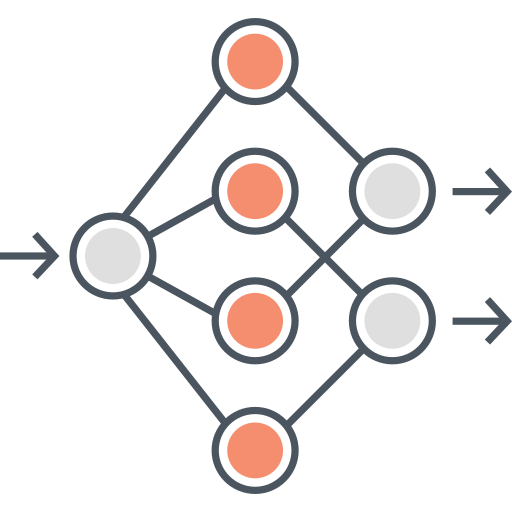
\includegraphics[scale=0.05]{nn.png}} (S);
        \draw[->] (S) -- node [midway,above] {} (LowRank);
        \node (mid) [right=of LowRank] {};
        \node (training) [above right=of mid] {$\|H_{\text{LR}} - G^TG \|^2$};
        \node (inference) [below right=of mid] {$H^{-1}_{\text{LR}}$};
        \draw[->] (LowRank) -- node [midway, above] {training} (training);
        \draw[->] (LowRank) -- node [midway, below] {inference} (inference);
    \end{tikzpicture}%}
    \caption{Flowchart for prec. training using low rank matrices}
    \label{fig:archi_nn_lowrank}
\end{figure}
$\rightarrow$ Did not give results (for a lack of structure ?)
\end{frame}

\begin{frame}{Deflation-like preconditioner}
$S =(s_1,\dots,s_r)$ has $r$ orthonormal columns ($S^TS = I_r$), 
and $(\lambda_1,\dots, \lambda_r) \in \mathbb{R}^{r}$, $\lambda_i > 0$
    \begin{align}
        H_{\text{defl}}(S, \lambda) &= I_n + \sum_{i=1}^r (\lambda_i- 1)s_is_i^T\\
        H^{-1}_{\text{defl}}(S, \lambda) &= I_n + \sum_{i=1}^r \left(\frac{1}{\lambda_i}- 1\right)s_is_i^T\\        
    \end{align}

    \begin{figure}
    \centering
    \resizebox{0.5\textwidth}{!}{    
        \begin{tikzpicture}[node distance = 1cm, thick]% 
        \node (1) {$x$};
        \node (S) [right=of 1] {$S(x)$, $\mu(x)$};
        \node (LowRank) [right=of S] {$\text{Deflation}(S(x), \mu(x))$};
        \draw[->] (1) -- node [midway,above] {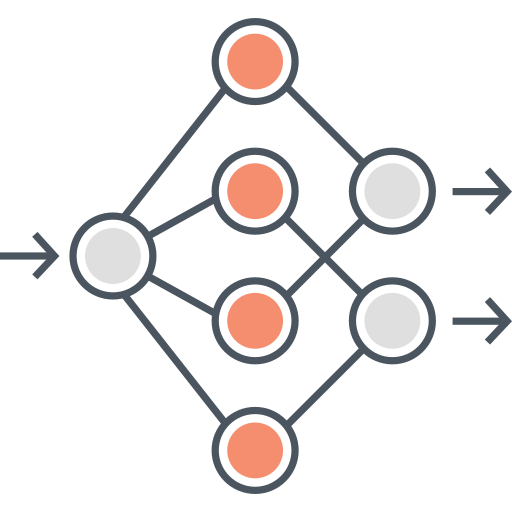
\includegraphics[scale=0.05]{nn.png}} (S);
        \draw[->] (S) -- node [midway,above] {} (LowRank);
        \node (mid) [right=of LowRank] {};
        \node (training) [above right=of mid] {$\|H_{\text{defl}} - G^TG \|^2$};
        \node (inference) [below right=of mid] {$H^{-1}_{\text{defl}}$};
        \draw[->] (LowRank) -- node [midway, above] {training} (training);
        \draw[->] (LowRank) -- node [midway, below] {inference} (inference);
    \end{tikzpicture}%}
    \caption{Flowchart for prec. training using deflation}
    \label{fig:archi_nn_defl}
\end{figure}
\end{frame}

\begin{frame}{Limited Memory Preconditioners \cite{tshimanga_class_2007,gratton_reduced_2011}}

Let $S = (s_1, \dots, s_r)$ be $r$ vectors of $\mathbb{R}^n$, $r\ll n$

{\small
\begin{equation}
    H^{-1}_{\text{LMP}}(S, \alert{AS}) = \left(\drawmatrix{I_n} - \drawmatrix[width=0.4]{S}\;\drawmatrix[height=0.4, width=0.4]{\Sigma}\;\drawmatrix[width=0.4]{\alert{AS}}^T\right)\left(\drawmatrix{I_n} - \drawmatrix[width=0.4]{\alert{AS}}\;\drawmatrix[height=0.4, width=0.4]{\Sigma}\;\drawmatrix[width=0.4]{S}^T\right) + \mu\drawmatrix[width=0.4]{S}\;\drawmatrix[height=0.4, width=0.4]{\Sigma}\;\drawmatrix[width=0.4]{S}^T
\end{equation}
\begin{equation}
    H_{\text{LMP}}(S, \alert{AS}) = \drawmatrix{I_n} + \drawmatrix[width=0.4]{\alert{AS}}\;\drawmatrix[height=0.4, width=0.4]{\Sigma}\; \drawmatrix[width=0.4]{\alert{AS}}^T - \frac{1}{\mu}\drawmatrix[width=0.4]{S}\;\drawmatrix[height=0.4, width=0.4]{\Gamma}\;\drawmatrix[width=0.4]{S}^T
\end{equation}
}


Given $S \in \mathbb{R}^{n \times r}$ and $\alert{AS} \in \mathbb{R}^{n \times r}$, we can construct $H_{\text{LMP}}$ and $H^{-1}_{\text{LMP}}$ directly, with nice properties (even though $\Sigma$ and $\Gamma$ require the inversion of a $r \times r$ matrix)

    Flexible preconditioners:
    \begin{itemize}
        \item $(s_1,\dots,s_r)$ eigenvalues of $A$ $\rightarrow$ Spectral Preconditioner
        \item $(s_1,\dots,s_r)$ CG descent vectors  $\rightarrow$ QN preconditioner
    \end{itemize}

\end{frame}
\begin{frame}{LMP construction using leap-forward NN}

\begin{figure}
    \centering
    \resizebox{0.8\textwidth}{!}{    
        \begin{tikzpicture}[node distance = 1cm, thick]% 
        \node (1) {$x$};
        \node (S) [right=of 1] {$S(x)$};
        \node (Spr) [right=of S] {$S'(x)$};
        \node (LMP) [right=of Spr] {$\text{LMP}(S(x), S'(x))$};
        \draw[->] (1) -- node [midway,above] {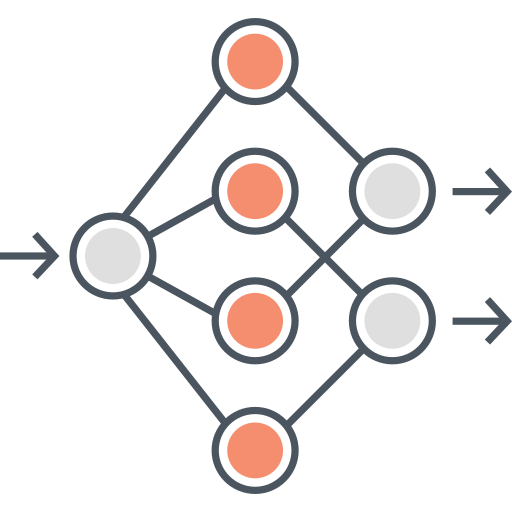
\includegraphics[scale=0.05]{nn.png}} (S);
        \draw[->] (S) -- node [midway,above] {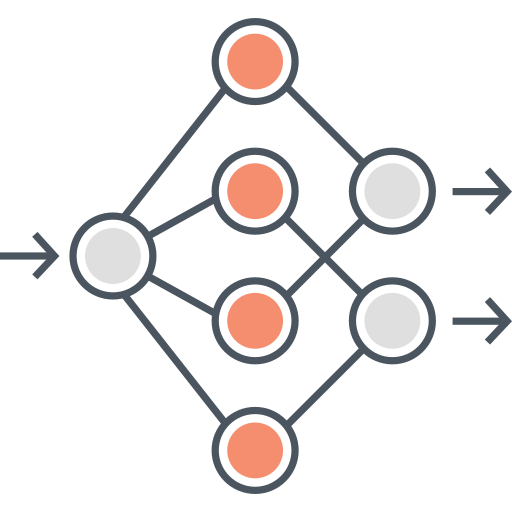
\includegraphics[scale=0.05]{nn.png}} (Spr);
        \draw[->] (Spr) -- node [midway,above] {} (LMP);
        \draw[->] (S) to [bend right] node [midway,below] {} (LMP);
        \node (mid) [right=of LMP] {};
        \node (training) [above right=of mid] {$\|H_{\text{LMP}} - G^TG \|^2$};
        \node (inference) [below right=of mid] {$H^{-1}_{\text{LMP}}$};
        \draw[->] (LMP) -- node [midway, above] {training} (training);
        \draw[->] (LMP) -- node [midway, below] {inference} (inference);
    \end{tikzpicture}%}
    \caption{Neural Network architecture for LMP}
    \label{fig:archi_nn_lmp}
\end{figure}
\textbf{But}: No particular structure imposed for $S'$ $\Rightarrow$ $\left(H_{\text{LMP}}(S, S')\right)^{-1} \neq H_{\text{LMP}}^{-1}(S, S')$

However: Good results were still obtained, even though the exact inverse is not used
\end{frame}

\begin{frame}{LMP: self adjoint variation}
    Force the self-adjointness of the operator $S \mapsto S'$ (which should be $=AS$) by constructing at the same time a low-rank approximation of $A$
\begin{figure}
    \centering
    \resizebox{0.8\textwidth}{!}{    
        \begin{tikzpicture}[node distance = .7cm, thick]% 
        \node (1) {$x$};
        \node (mid) [right=of 1] {};
        \node (S) [above right=of mid] {$S(x)$};
        \node (L) [below right=of mid] {$L(x)$};
        \draw[->] (1) -- node [midway,above] {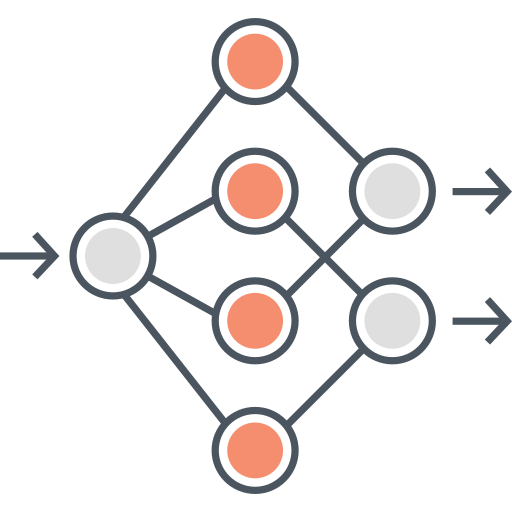
\includegraphics[scale=0.05]{nn.png}} (S);
        \draw[->] (1) -- node [midway,below] {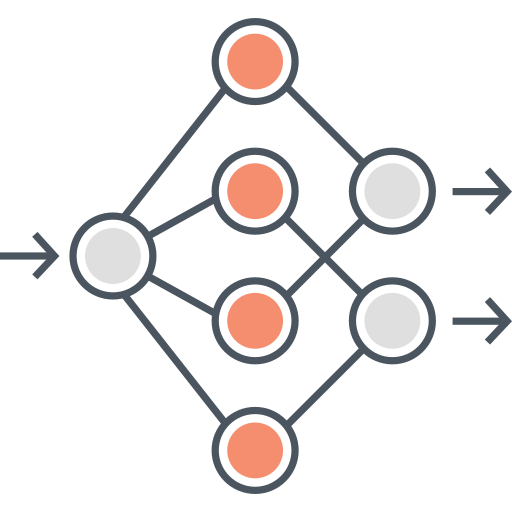
\includegraphics[scale=0.05]{nn.png}} (L);
        \node (Spr) [right=of L] {$S'(x) = \left(I_n + L(x)L(x)^T\right)S(x)$};
        \draw[->] (L) -- (Spr);
        \node (LMP) [above right= of Spr] {$\text{LMP}(S(x), S'(x))$};
        \draw[->] (Spr) -| node [midway,above] {} (LMP);
        \draw[->] (S) -| node [midway,above] {} (LMP);
        \draw[->] (S) -| node [midway,above] {} (Spr);
        \node (mid) [right=of LMP] {};
        \node (training) [above right=of mid] {$\|H_{\text{LMP}} - G^TG \|^2$};
        \node (inference) [below right=of mid] {$H^{-1}_{\text{LMP}}$};
        \draw[->] (LMP) -- node [midway, above] {training} (training);
        \draw[->] (LMP) -- node [midway, below] {inference} (inference);
        
\end{tikzpicture}%}
    \caption{Neural Network architecture for symmetric LMP}
    \label{fig:archi_nn_lmp_sym}
\end{figure}
with $L(x) \in \mathbb{R}^{n \times n'}$
\end{frame}

\begin{frame}{Training setting: Dataset}
For an input $x$, we assume to have access to $G(x)^TG(x)$,

$\rightarrow$ Training dataset: $\mathcal{D} = \{(\underbrace{x_i}_{\in \mathbb{R}^n}, \underbrace{G(x_i)^TG(x_i))}_{\in \mathbb{R}^{n\times n}}\}$

\begin{itemize}
    \item Very large in memory when dimension increases
    \item We access $G$ only as an operator: $\mathrm{TL}(x, z) = G(x) \cdot z$
    \item Same for adjoint: $\mathrm{Adj}(x, y) = G(x)^T \cdot y$
    \item Constructing $G(x)$ would require $n$ call to the TL
\end{itemize}
\end{frame}
\begin{frame}{Less storage intensive solution: Iterable Datasets}
    Estimate the $L_2$ norm using random Gaussian vectors:
    \begin{block}{Matrix norm estimation}
    For a matrix $M$, and $z \sim \mathcal{N}(0, I)$
    \begin{equation}
        \mathbb{E}_Z\left[\|Mz\|^2_2\right] = \|M\|^2_{\mathrm{F}}
        \end{equation}
    \end{block}
    $\rightarrow$ Iterable Dataset: $\mathcal{D} = \{(\underbrace{x_i}_{\in \mathbb{R}^n}, \underbrace{Z_i}_{\in \mathbb{R}^{n \times n_Z}}, \underbrace{G(x_i)^TG(x_i)Z_i}_{\in \mathbb{R}^{n\times n_Z}})_i\}$ where $Z_i$ has $n_Z$ columns iid $\mathcal{N}(0, I)$
    The loss for a data point becomes then
    \begin{equation}
        \mathcal{L}_{\theta}(x_i) = \sum_{j=1}^{n_Z} \| H_{\theta}(x_i) z_i^j - G^T(x_i)G(x_i)z_i^j \|^2_2
    \end{equation}
    and we can generate the dataset "on the fly", and train the network in an online manner
\end{frame}
% \begin{frame}{Regularization ?}
% \begin{block}{Ortho(gonal/normal): Gram matrix}
%     Let $S = \Big( s_1 \big\rvert s_2 \big\lvert \dots \big\rvert s_r \Big)$
%     \begin{equation}
%         K = S^TS \text{ has general term } K_{i,j}= \langle s_i, s_j \rangle = s_i^Ts_j
%     \end{equation}
%     \begin{align}
%         R_{\text{orthogonal}}(S) &\propto \Large\lVert\drawmatrixset{bbox style={fill=red!10}}\drawmatrix[lower, size=.8, bbox height=1, bbox size=1.1, offset height=0.3]K\Large\rVert \\
%         R_{\text{orthonormal}}(S) &\propto \| K - I_r\|^2
%     \end{align}
% \end{block}
% \begin{block}{Symmetry of the LMP}
%     \begin{equation}
%         R_{\text{sym}}(H) \propto \|H - H^T\|^2
%     \end{equation}
% \end{block}
% \end{frame}

\begin{frame}{Regularization}
\begin{block}{$A$-conjugacy}
    Let $S = \Big( s_1 \big\rvert s_2 \big\lvert \dots \big\rvert s_r \Big)$. The column vectors of $S$ are $A$-conjugate when $S^TAS$ is diagonal

    Since $S'$ is supposed to be $AS$
    \begin{equation}
        K = S^TS' \text{ has general term } K_{i,j}= \langle s_i, s'_j \rangle = s_i^Ts'_j \approx s_i^TAs_j
    \end{equation}
    \begin{align}
        R_{\text{conjugacy}}(S) &\propto \Large\lVert\drawmatrixset{bbox style={fill=white!10}}\drawmatrix[banded, dashed,fill=red!10, bandwidth=0.2]K\Large\rVert
    \end{align}
\end{block}
But we may also add regularization on symmetry of the LMP, orthonormalization of the outputs etc...
\end{frame}
% \begin{frame}{LMP: $\dim=40$, rank=8}
%     \includegraphics<1>[width=\textwidth]{img/40_rk8_nu0.png}
% \end{frame}

\section{Example on Lorenz96 (40D)}
\begin{frame}{Statistics}
\begin{figure}
    \centering
    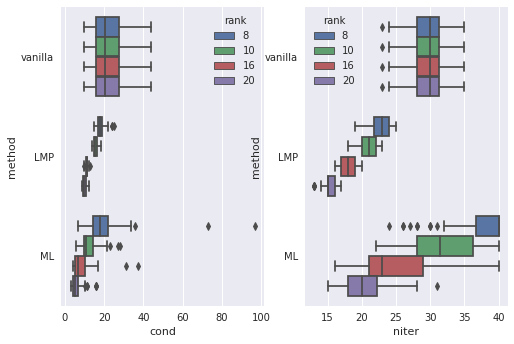
\includegraphics[scale=0.4]{img/boxplot.png}
    \caption{Statistics on inference model}
    \label{fig:stats_inference}
\end{figure}   
\end{frame}
\begin{frame}{Inner loop CV: leap forward LMP $(r=20)$}
Comparison:
\begin{itemize}
    \item \textcolor{blue}{Baseline}: no preconditioner
    \item \textcolor{red}{Spectral LMP}: computation of eigenvectors for every inner loop
    \item \textcolor{green}{ML-LMP}: preconditioned inner loop using "leap forward" LMP
\end{itemize}
\begin{centering}
\begin{figure}
    \centering
    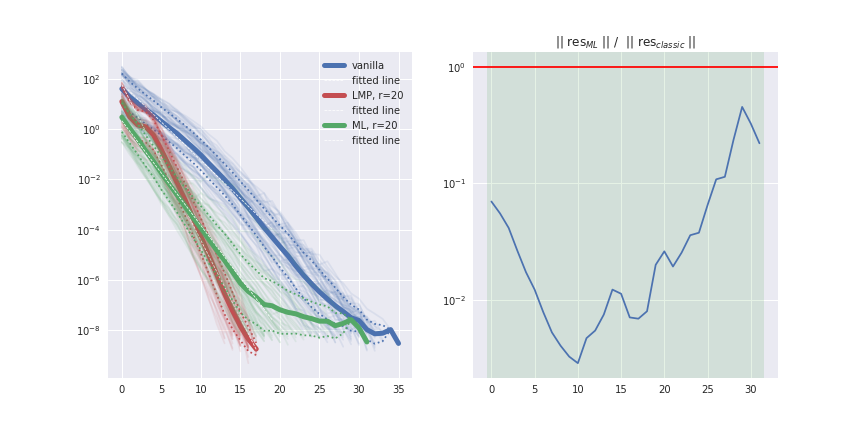
\includegraphics[width=.7\linewidth]{img/40-inv-rank-20-composite-box_rate_cv_inner_loop.png}
    \caption{Inner loop convergence}
    \label{fig:inner_loop_cv}
\end{figure}   
\end{centering}
\end{frame}
\begin{frame}{Inner loop CV: leap forward LMP $(r=16)$}
Comparison:
\begin{itemize}
    \item \textcolor{blue}{Baseline}: no preconditioner
    \item \textcolor{red}{Spectral LMP}: computation of eigenvectors for every inner loop
    \item \textcolor{green}{ML-LMP}: preconditioned inner loop using "leap forward" LMP
\end{itemize}
\begin{centering}
\begin{figure}
    \centering
    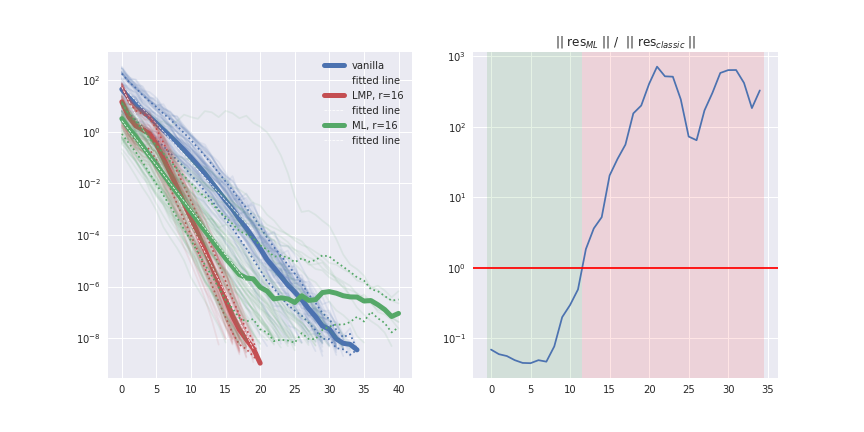
\includegraphics[width=.7\linewidth]{img/40-inv-rank-16-white-cottage_rate_cv_inner_loop.png}
    \caption{Inner loop convergence}
    \label{fig:inner_loop_cv2}
\end{figure}   
\end{centering}
\end{frame}
\begin{frame}{Inner loop CV: self adjoint LMP $(r=20)$}
Comparison:
\begin{itemize}
    \item \textcolor{blue}{Baseline}: no preconditioner
    \item \textcolor{red}{Spectral LMP}: computation of eigenvectors for every inner loop
    \item \textcolor{green}{ML-LMP}: preconditioned inner loop using self adjoint LMP
\end{itemize}
\begin{centering}
\begin{figure}
    \centering
    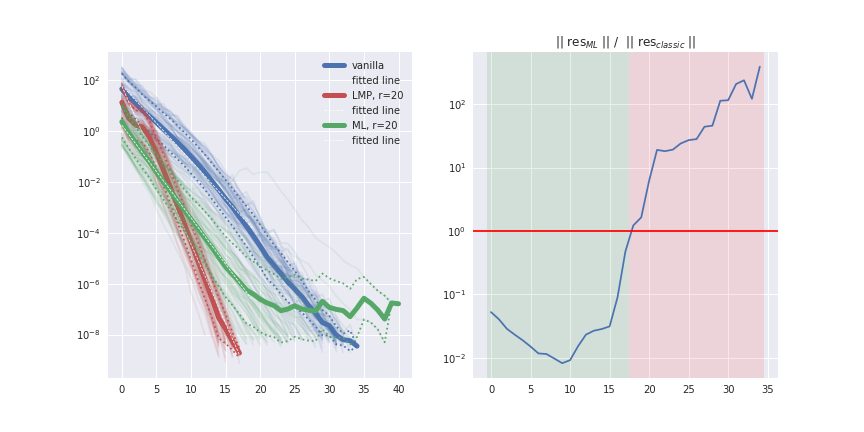
\includegraphics[width=.7\linewidth]{img/40-inv-rank-20-absolute-doorjamb_rate_cv_inner_loop.png}
    \caption{Inner loop convergence}
    \label{fig:inner_loop_cv3}
\end{figure}   
\end{centering}
\end{frame}

%{\setbeamercolor{palette primary}{fg=white, bg=black}

\begin{frame}{Work in progress / Open questions}
    \begin{itemize}
        \item Apply this preconditioner in 4D-Var \checkmark
        \item Output both $S_{\theta}$ and $AS_{\theta}$ \checkmark
        \item How to train without explicit access to A \faGears
        \begin{itemize}
            \item Online training ?
            \item Use information of $G^T(x)G(x)Z$ (Link to REVD \cite{dauzickaite_randomised_2021})
        \end{itemize}
        \end{itemize}
    \begin{itemize}
        \item How to get more consistent results in 4D-Var ? \faGears
        \item Which regularization to use \faGears
        \item Apply to system with worse conditioning (QG) and/or higher dimension (QG / KS) \faGears
    \end{itemize}    
        \begin{itemize}
        \item Exploit conditioning using the prior ("$(B + G^TG) \rightarrow (I + \tilde{G}^T\tilde{G})$") \faQuestionCircle
        \item Extension to weak 4DVar  \faQuestionCircle
        \item Adapt to time-varying observation operators  \faQuestionCircle
        \end{itemize}
\end{frame}




\begin{frame}[allowframebreaks]{References}
  \bibliography{bibzotero}
  \bibliographystyle{apalike}
\end{frame}

\end{document}
